\chapter{Experiments}
There are 8 experiments in this thesis which can be classified into four parts: basic models, mix data model, fine-tuning models, and increment fine-tuning models. In the first part, I train models in order to compare with other experiments and choose some parameters. In mix-data part, I try to train models using both source and target data. When it comes to fine-tuning part, I use target data to fine-tune source model. Finally, I try to add target data gradually into fine-tuned model.

\section{Cross Validation}
I use cross validation to validate my model and divide training/validation/testing sets. Cross validation is validation techniques for assessing how the results of a model will generalize to an independent dataset and estimating how accurately a predictive model will perform in practice. I divide dataset into 10 subsets. Then I choose one to be testing set while the rest part is training set and validation set. For the rest 9 subset, I choose 10 \% to be validation set and the rest 90 \% is training set. The two tables below shows how we divide training/validation/testing sets for source data and target data.


\begin{figure}[H]
    \hfil
    \begin{minipage}[t]{0.9\textwidth}
        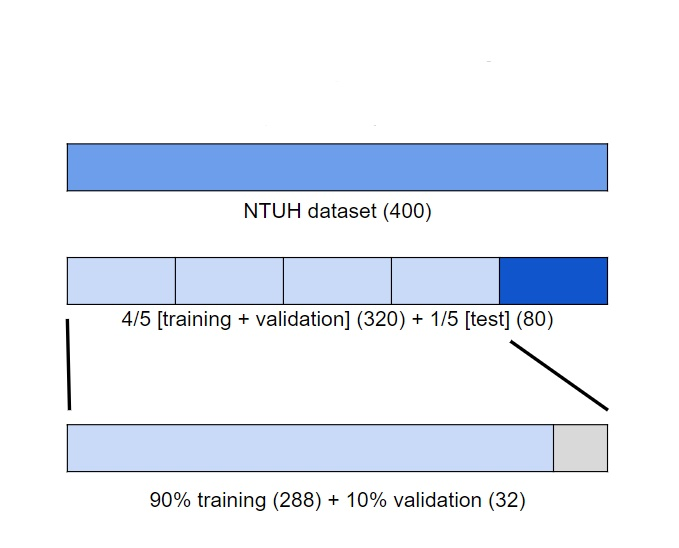
\includegraphics[width=\textwidth]{fig/cross.png}
        \caption{\label{fig:parallel1} AUC for Mix Source Data and Target Data}
    \end{minipage}
    \hfil
\end{figure}
 
 \begin{table}[H]
\centering
\caption{training/validation/testing set (10 folder)}
\begin{tabular}{|l|l|l|l|l|} 
\hline
~            & source H & source T & target H (tcia) & target T (msd)  \\ 
\hline
train        & 324      & 324      & -               & -               \\ 
\hline
validation   & 36       & 36       & -               & -               \\ 
\hline
source test  & 40       & 40       & 0               & 0               \\ 
\hline
target test~ & 0        & 0        & 8               & 28              \\
\hline
\end{tabular}
\end{table}
\begin{table}[H]
\centering 
\caption{training/validation/testing set (B) (10 folder)}
\begin{tabular}{|l|l|l|l|l|} 
\hline
amount of data   & tar H (train) & tar T (train) & tar H (val) & tar T (val)  \\ 
\hline
50       & 17      & 57      & 2               & 6               \\ 
\hline
100 & 33       & 114       & 4               & 13               \\ 
\hline
150& 50       & 171       & 6               & 19               \\ 
\hline
200&66        & 228        & 7               & 25              \\
\hline
250& 50       & 171       & 6               & 19               \\ 
\hline
300&66        & 228        & 7               & 25              \\
\hline
\end{tabular}
\end{table}
 ~\\
\section{Basic Models}
In this part, I train models in order to compare with other experiments and choose parameters for other experiments.
\subsection{Train Models Using Only Source Data (B1)}
First, I want to calculate the prediction results if the model is only consider about source data. The results will compare with other experiment results to see how much other methods will improve. The amount of target data fixes 0.
\subsection{Train Models Using Only Target Data (B2)}
I want to calculate the prediction results if the model is only consider about target data. I want to know if how much data I need to get a sufficiently nice model. The amount of target data varies from 50 to 300.
\subsection{Choose the Number of Fixed Layers in Fine-tuning Experiments (B3)}
All experiments in this thesis use a simplified VGG model for training,  sometimes it's better to fix some layers since the target dataset is small for fine-tuning. The goal of this experiment is to find the number of fixed layers in fine-tuning experiments. The amount of target data fixes 300.
~\\
\section{Mix Data Models}
\subsection{Mix Data Models (M1)}
In this part, we mix source and target data to train model. The amount of target data varies from 50 to 300.
~\\
\section{Fine-Tuning Models}
\subsection{Fine-Tuning Models (M2)}
In this part, I fine-tune the model trained in (B1) using target data. I fix 3 layers in this experiments. The amount of target data varies from 50 to 300.
~\\
\section{Increment Fine-Tuning Models}
Suppose we get an unlabeled target dataset, we want to first label some data that best improve the model performance and use them to fine-tune model. If the performance is not good enough, we need to repeat all steps and fine-tune model using another selected dataset.
\subsection{Fine-tuning Using Selected Target Data (I1)}
We use selected subset to fine-tune the model. The number of patients in selected subset varies from 30 to 150.

\subsection{Fine-tuning Using Random Target data (I2)}
We replace the select method to random selection to valid that the selection method really works. The number of patients in selected subset varies from 30 to 150.

\subsection{Gradually Fine-tuning Using Selected Target Data (I3)}
We gradually add selected subset of target data until all target data is used to observe the performance. The amount of target data varies from 50 to 300.